%!TEX root = ../main.tex

\newpage
\section*{Tables and Figures}

% Tables

  \begin{table}[h]
    \centering
    \small
    \begin{tabular}{|c|c|c|}
      \hline
      \textbf{Process} & \textbf{Tool} & \textbf{Parameters} \\
      \hline
      Denoising and Clustering & Dada2/Deblur & default \\
      Taxonomy Assignment & \ac{ncbi} with Blast & RefSeq database \\
      OTU Processing & Based on statistical power & Dynamic cutoff \\
      Network Inference & Consensus method & - \\
      \hline
    \end{tabular}
    \caption{Default tools and parameters for the pipeline}
    \label{tab:default_options}
  \end{table}

  \begin{table}[h]
    \centering
    \small
    \begin{tabular}{|c|c|c|}
      \hline
      \textbf{Module} & \textbf{Tool} & \textbf{References} \\
      \hline
      Denoising and Clustering & Closed reference & \cite{rognesVSEARCHVersatileOpen2016,bolyenReproducibleInteractiveScalable2019} \\
      Denoising and Clustering & Open reference & \cite{rognesVSEARCHVersatileOpen2016,bolyenReproducibleInteractiveScalable2019} \\
      Denoising and Clustering & De novo & \cite{rognesVSEARCHVersatileOpen2016,bolyenReproducibleInteractiveScalable2019} \\
      Denoising and Clustering & Dada2 & \cite{Callahan2016} \\
      Denoising and Clustering & Deblur & \cite{Amir2017,bolyenReproducibleInteractiveScalable2019} \\
      \hline
      Chimera checking & Uchime & \cite{rognesVSEARCHVersatileOpen2016,bolyenReproducibleInteractiveScalable2019} \\
      Chimera checking & Remove bimera & \cite{Callahan2016} \\
      \hline
    \end{tabular}
    \caption{Tools used in the DC module}
    \label{tab:dc_tools}
  \end{table}

  \begin{table}[h]
    \centering
    \small
    \begin{tabular}{|c|c|c|}
      \hline
      \textbf{Module} & \textbf{Tool/Database} & \textbf{References} \\
      \hline
      Query tool & Blast & \cite{camachoBLASTArchitectureApplications2009,bokulichOptimizingTaxonomicClassification2018} \\
      Query tool & Naive bayes classifier & \cite{bokulichOptimizingTaxonomicClassification2018} \\
      \hline
      Database & Greengenes & \cite{DeSantis2006} \\
      Database & SILVA & \cite{Quast2012} \\
      Database & NCBI RefSeq & \cite{Sayers2009} \\
      \hline
    \end{tabular}
    \caption{Tools used in the TA module}
    \label{tab:ta_tools}
  \end{table}

  \begin{table}[h]
    \centering
    \small
    \begin{tabular}{|c|c|c|}
      \hline
      \textbf{Module} & \textbf{Tool/Database} & \textbf{References} \\
      \hline
      Booststrap & \texttt{fastspar\_bootstraps} v1.0 & \cite{Watts2018} \\
      Booststrap & \texttt{fastspar\_pvalues} v1.0 & \cite{Watts2018} \\
      \hline
      Direct & \ac{spieceasi} v1.1.2 & \cite{Kurtz2015} \\
      Direct & FlashWeave.jl v0.18.1 & \cite{tackmannRapidInferenceDirect2019} \\
      Direct & \ac{cozine} v1.0 & \cite{haCompositionalZeroinflatedNetwork2020a} \\
      Direct & \ac{harmonies} v1.0 & \cite{jiangHARMONIESHybridApproach2020} \\
      Direct & \ac{spring} v1.0.4 & \cite{yoonMicrobialNetworksSPRING2019} \\
      Direct & \ac{mldm} v1.1 & \cite{Yang2017} \\
      \hline
      Correlation & FastSpar (\ac{sparcc}) v1.0 & \cite{Watts2018} \\
      Correlation & Pearson & - \\
      Correlation & Spearman & - \\
      Correlation & propr v2.1.2 & \cite{quinnProprRpackageIdentifying2017} \\
      \hline
    \end{tabular}
    \caption{Tools used in the NI module}
    \label{tab:ni_tools}
  \end{table}



% Figures

  \begin{figure}[H]
    \centering
    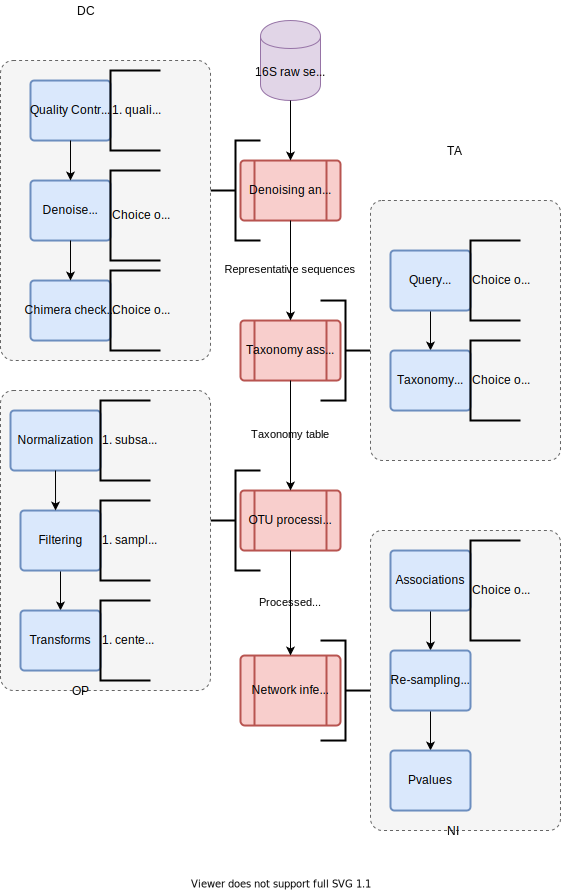
\includegraphics[width=0.75\linewidth]{figure1.pdf}
  \end{figure}
  \begin{figure}[H]
    \centering
    \caption{
      \textbf{The workflow of the microbial co-occurrence analysis pipeline}.
      The steps can be grouped into four major groups: \textbf{(DC)} \textbf{D}enoising and \textbf{C}lustering, \textbf{(TA)} \textbf{T}axonomy \textbf{A}ssignment, \textbf{(OP)} \textbf{O}TU or ESV \textbf{P}rocessing, and \textbf{(NI)} \textbf{N}etwork \textbf{I}nference.
      Each step incorporates several processes, each of which in turn have several alternate algorithms for the same task (indicated by the text to the right of the blue boxes).
      The text along the arrows describes the data that is being passed from one step to another. For details on each process and data types, see Methods.
    }
    \label{fig:figure1}
  \end{figure}

  \FloatBarrier
  \newpage

  \begin{figure}[H]
    \centering
    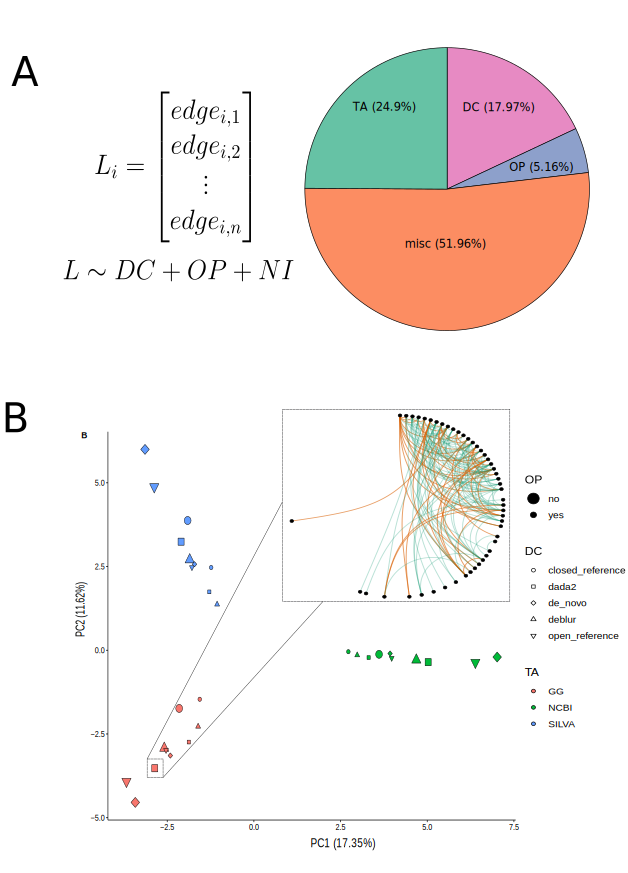
\includegraphics[width=1.0\linewidth]{figure2.pdf}
  \end{figure}
  \begin{figure}[H]
    \centering
      \caption{
      \textbf{The choice of database contributes to the most variance in the networks}.
      \textbf{(A)} The total relative variance in the networks contributed by the DC, TA and OP steps of the pipeline (right) and the linear model used to calculate the relative variance (left), see the Methods section for details.
      \textbf{(B)} All combinations of inferred networks are shown as points on a PCA plot.
      The color of the points corresponds to the taxonomy database, the shape corresponds to the denoising/clustering method and the size corresponds to whether low abundance OTUs were removed or not.
      \textbf{(B inset)} The network generated using DC=dada2, TA=GG, OP=no and NI=SPARCC and represents the particular point shown (big red square).
      The points on the PCA plot can be separated based on the TA step and the differences due to the DC and OP steps are comparatively not as significant.
    }
    \label{fig:figure2}
  \end{figure}
  \FloatBarrier
  \newpage

  % TODO: Describe the datasets being shown here clearly. In the caption + figure legends (if necessary) and in the text
  \begin{figure}
    \centering
    \includegraphics[width=\textwidth]{figure3.pdf}
    \caption{
      \textbf{The representative sequences generated by the different denoising/clustering methods are very similar but differ in the sequences that are in low abundance.}
      \textbf{(A)} The average weighted UniFrac distance between the representative sequences shows that the representative sequences and their compositions are fairly identical between the methods,
      \textbf{(B)} The relatively larger average unweighted UniFrac distance indicates that methods differ in their identification of sequences of low abundance,
      \textbf{(C, D)} The distributions of the average weighted UniFrac distance between the expected sequence profile and the calculated sequence profile in mock datasets.
      \textbf{(D)} The distributions of the average unweighted UniFrac distance show that dada2 and Deblur were the best performing methods in most of the datasets.
    }
    \label{fig:figure3}
  \end{figure}
  \FloatBarrier
  \newpage

  \begin{figure}[H]
    \centering
    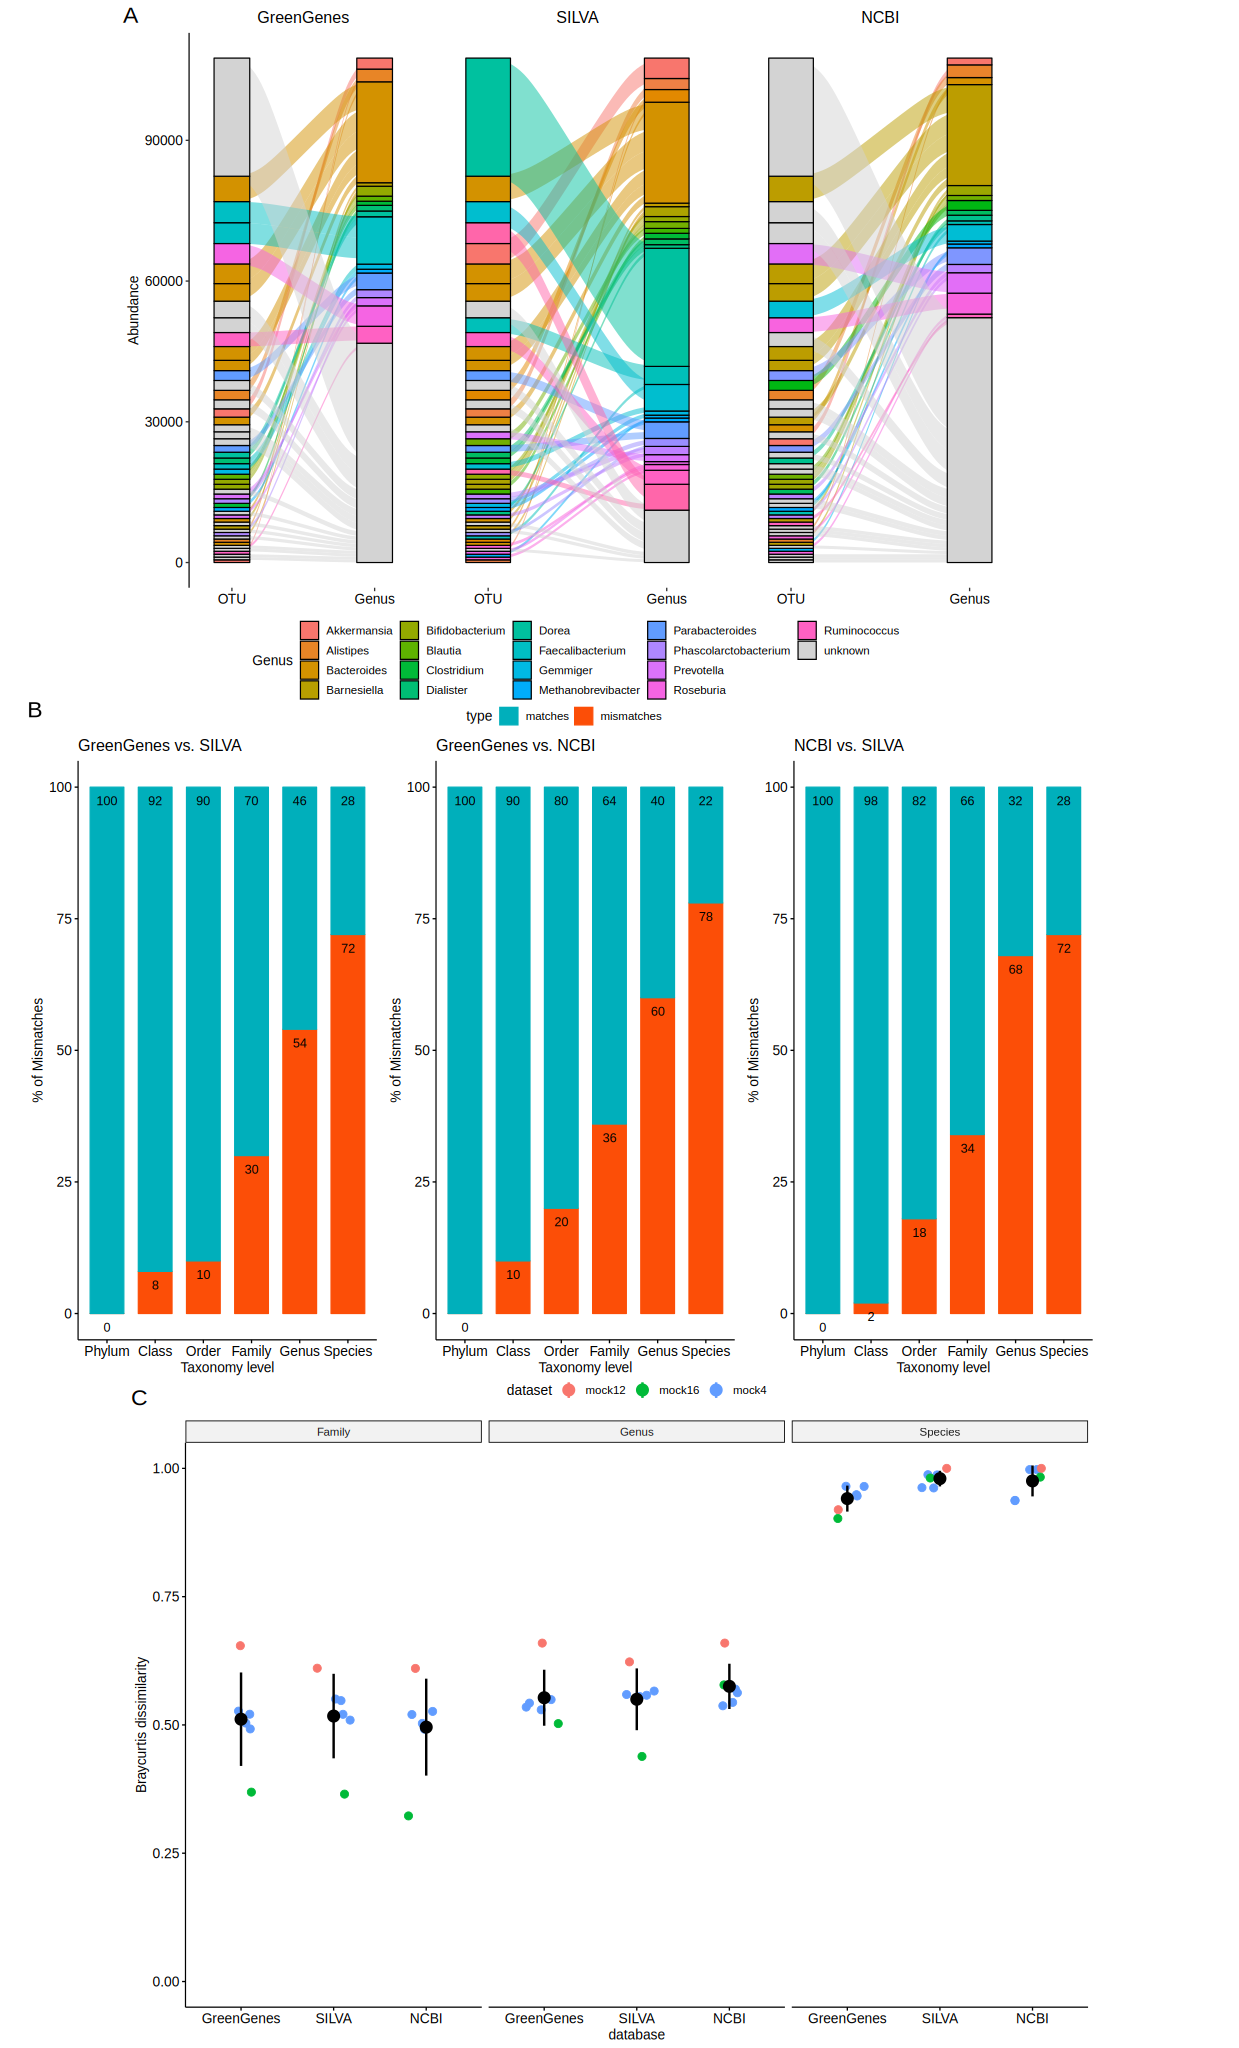
\includegraphics[width=0.9\textwidth,height=1.2\textwidth]{figure4.pdf}
  \end{figure}
  \begin{figure}[H]
    \centering
    \caption{
      \textbf{Taxonomic reference databases vary widely in terms of their taxonomy assignments.}
      \textbf{(A)} The assignment of the top 50 representative sequences to their respective taxonomies using the three different reference databases shows how the same sequences are assigned to different Genus.
      \textbf{(B)} The percentage of \ac{otu}s assigned to the same taxonomic label when using different reference databases.
      The percentage of mismatches decrease at higher taxonomic levels but even at the Phylum level there exists around 10\% of mismatches.
      \textbf{(C)} The Bray-Curtis dissimilarity between the expected taxonomy profile and calculated taxonomy profile in the mock datasets shows that there is no singular best choice of database for every dataset.
    }
    \label{fig:figure4}
  \end{figure}
  \FloatBarrier
  \newpage


  \begin{figure}[H]
    \centering
    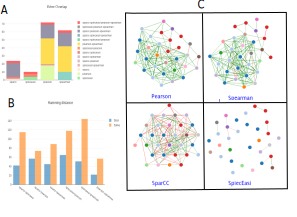
\includegraphics[width=0.9\textwidth]{figure5.pdf}
  \end{figure}
  \begin{figure}[H]
    \centering
    \caption{
      \textbf{Networks generated using different network inference methods show notable differences both in terms of edge-density and connectivity}.
      \textbf{(A)} The six different networks generated by the different network inference methods are very dissimilar.
      The green links are positive associations and the orange links are negative associations.
      A threshold of 0.3 was set for the methods that infer pairwise correlations (\ac{sparcc}, Spearman, Pearson) and no threshold was set for the other methods.
      \textbf{(B)} The node overlap Upset plot~\cite{Lex} indicates that all the networks have a large number of common nodes involved in connections.
      Whereas, \textbf{(C)} The edge overlap Upset plot shows that a very small fraction of these connections are actually shared.
    }
    \label{fig:figure5}
  \end{figure}
  \FloatBarrier
  \newpage

  \begin{figure}[h]
    \centering
    \includegraphics[width=1.0\linewidth]{figure6.pdf}
    \caption{
      The precision and sensitivity of the inferred networks on the synthetic data.
    }
    \label{fig:figure6}
  \end{figure}
  \FloatBarrier
  \newpage

  \begin{figure}[h]
    \centering
    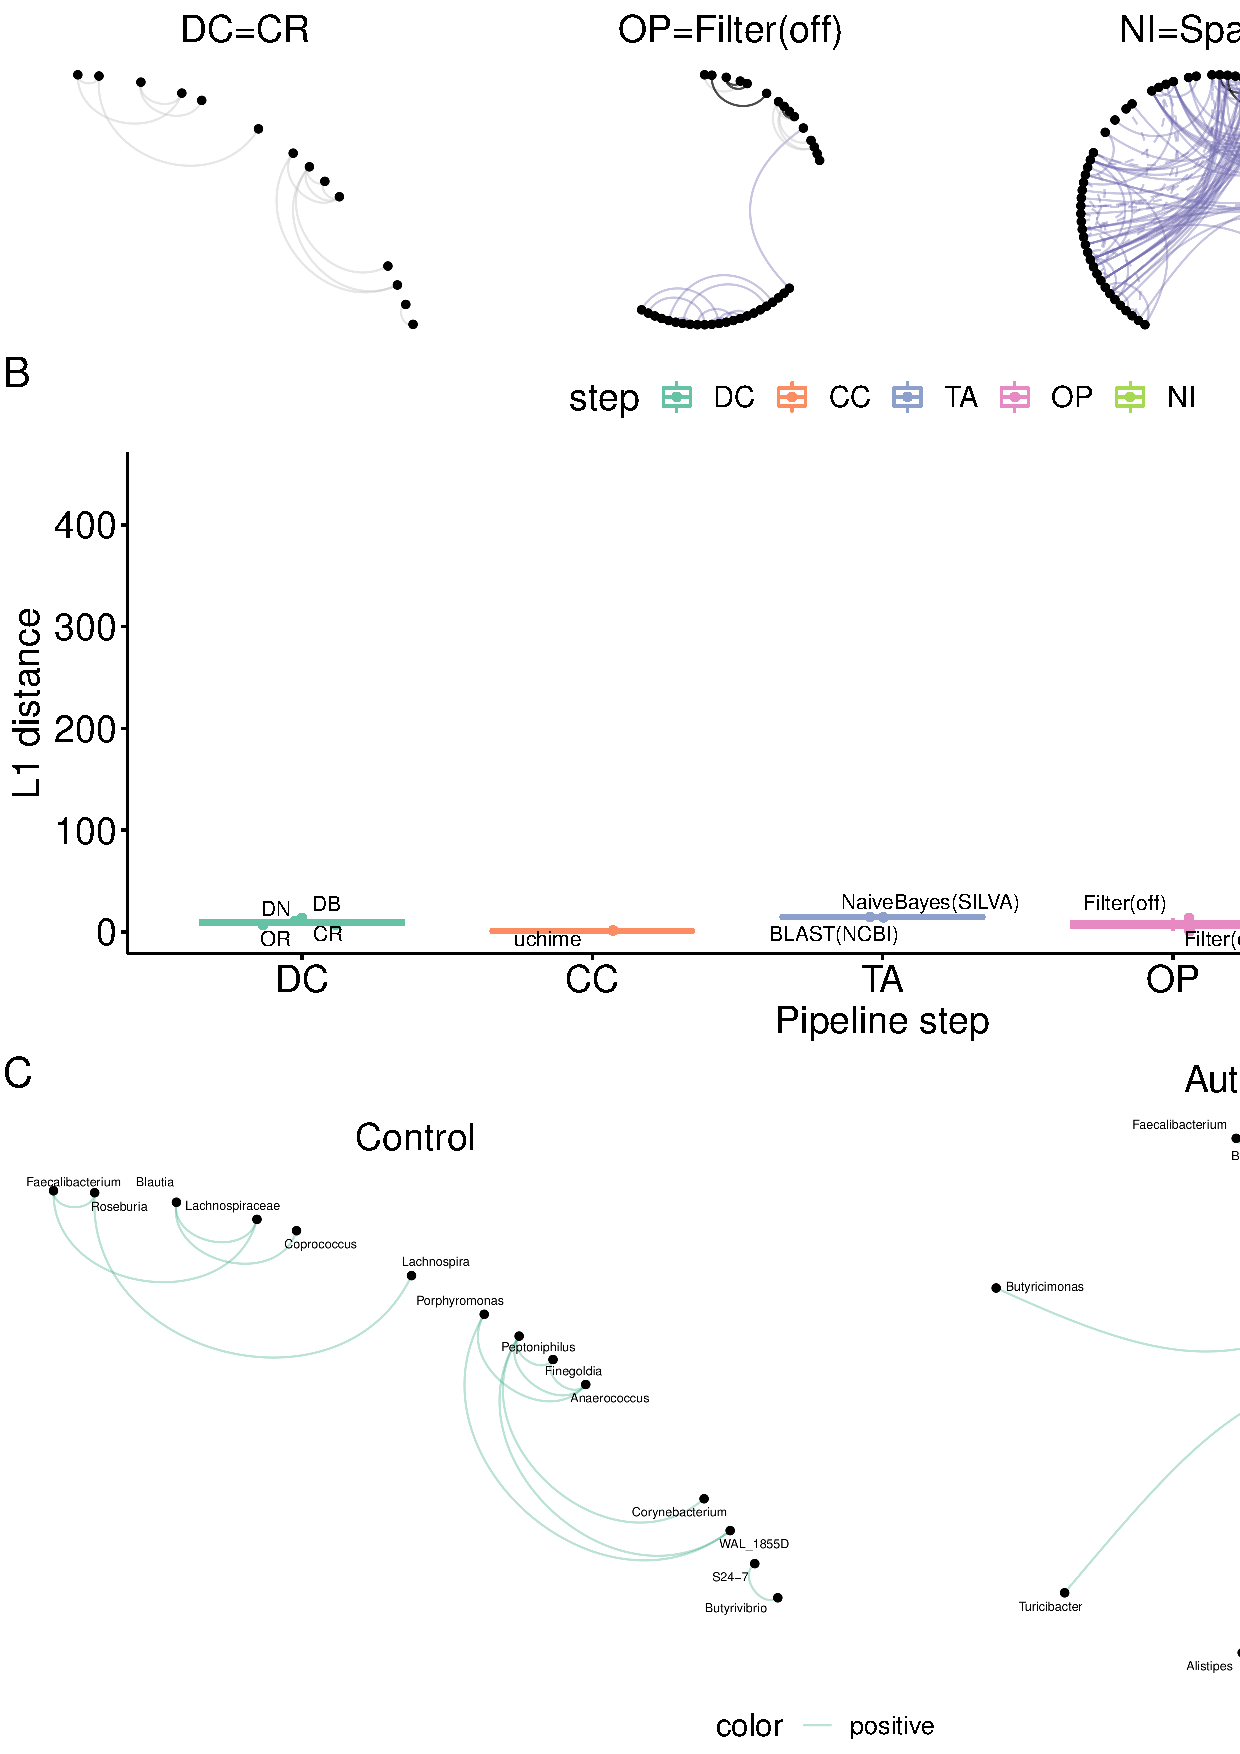
\includegraphics[width=0.85\linewidth]{figure7.pdf}
    \caption{
      \textbf{Network inference and taxonomic assignment have the highest influence on the inferred network structures.}
      \textbf{(A)} The network constructed using the default pipeline parameters (DC=\ac{dada2}, TA=\ac{ncbi}, OP=on, NI=\ac{sparcc}) is compared with networks generated when one of the steps use a different tool.
      The common connections (common with the default network) are in black, connections unique to the network are colored purple and connections in the default network but not present in the current network are gray.
      \textbf{(B)} The L1 distance between the networks generated by changing one step of the default pipeline and the network generated using the default parameters.
    }
    \label{fig:figure7}
  \end{figure}
